\section*{Neuroimaging}
In order to investigate the workings of the brain, there is a wide variety of tools that give us specific types of information. We can investigate at the micro scale, the level of the individual neuron, or the macro scale, the level of thousands of neurons firing at the same time. But when we zoom in to the micro scale, we can only measure a very small subset of the approximately 86 billion neurons in the human brain \cite{Herculano-Houzel2009}. Additionally, if this has to be done in a living animal, this is a very invasive procedure and thus is almost impossible in humans. Macro scale procedures are less invasive and measure electric or magnetic fields outside the brain with electroencephalography (EEG) or magnetoencephalography (MEG). However, it requires thousands of neurons to fire synchronously to pick up such a signal and gives little insight about the spatial location in the brain. Another technique that can image the brain is MRI. While it does not measure neuronal activity directly, and is not as fast as (M/E)EG, it gives highly detailed three dimensional images of the brain. MRI is not nearly specific enough for the micro scale, but may just be able to pick up information from the organisational units that are formed by neurons: the cortical layers and cortical columns. In this thesis, we explore the possibility of using MRI for the meso scale, the intermediate between the neurons and the networks. We push the limits of fMRI analysis to prepare functional MRI (fMRI) for higher spatial resolution, such that we reach the level of the cortical layers (See Figure~\ref{fig:spatiotemporal}). This could teach us more about how neuronal networks communicate with each other and together accomplish complex the tasks of which the brain is capable. 
\begin{figure}[H]
	\centering
	\includegraphics[width=0.8\textwidth, clip=true]{./Chapters/01_Introduction/Images/SpatioTemporalResolution}
	\caption{The temporal and spatial resolution of neuroimaging methods. By and large, methods of higher spatial resolution are more invasive. In this thesis, we tried to use the non-invasive technique of fMRI to cross the boundary of layer specificity. Picture recreated after Sejnowski et al. (2014) \cite{Sejnowski2014}.}
	\label{fig:spatiotemporal}
\end{figure}

\section*{Cortical layers}
The grey matter of the cortex is a thin shell of approximately 3 mm \cite{Zilles1990} around the white matter. The white matter consists of long fiber tracts that relay signals from one brain area to another, but it is mainly the grey matter where computations are being performed. The grey matter itself consists of several shells as well, cortical layers (see Figure~\ref{fig:layers}), that are likely to have functionally distinct roles.
\begin{figure}[!ht]
	\centering
	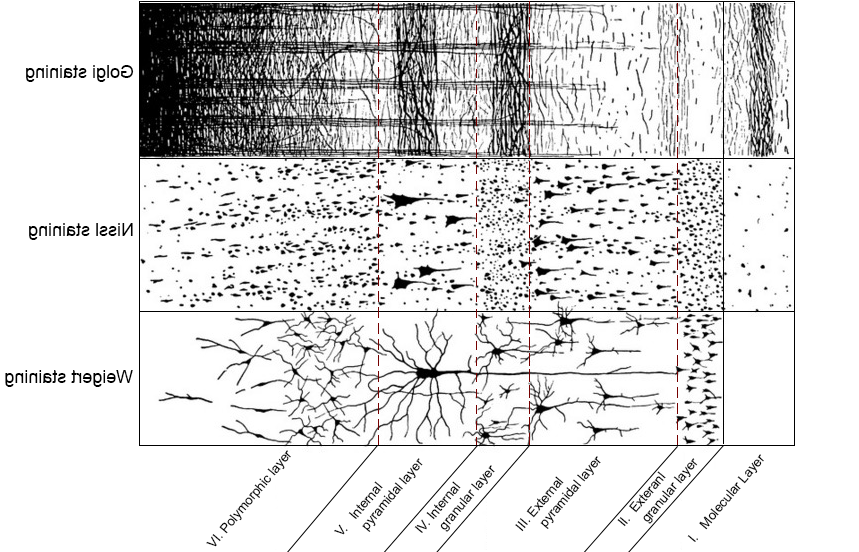
\includegraphics[width=0.8\textwidth, clip=true]{./Chapters/01_Introduction/Images/Layers}
	\caption{\cite{Brodman1909} }
	\label{fig:layers}
\end{figure}
The specifics of the performed computations are largely unknown, but in general, three types of information can be dissociated according to the predictive coding framework \cite{Friston2010}. At the fundamental level, the brain continuously makes predictions, compares it to (sensory) input, and the difference is called the prediction error. This is a never ending recurrent process of updating knowledge based on new information. The different roles within the predictive coding framework can largely be associated with the cortical layers. In principle, ascending (feed forward, e.g. `I \emph{see} an apple') and descending connections (feedback, e.g. `I \emph{imagine seeing} an apple') are distinguished \cite{Rockland1979} and can be related to hierarchical ranks of processing \cite{Barone2000}. For a given layer $i$ in the hierarchy, it receives feed forward input that target layer 4 and to a lesser extent layer 5 \cite{Constantinople2013} and they predominantly originate from supragranular layers (see Figure~\ref{fig:layerprocessing}). On the other hand, feedback connections from higher areas terminate primarily in layers 1 and 5, but avoid layer 4 \cite{Anderson2009}. The differential contribution is not well established \cite{Shipp2013}. This `canonical microcircuit' describes the excitatory relay of information within the cortex. With its link to the predictive coding, it can provide a more mechanistic understanding of the computations in the brain \cite{Shipp2016}.
\begin{figure}[!ht]
	\centering
	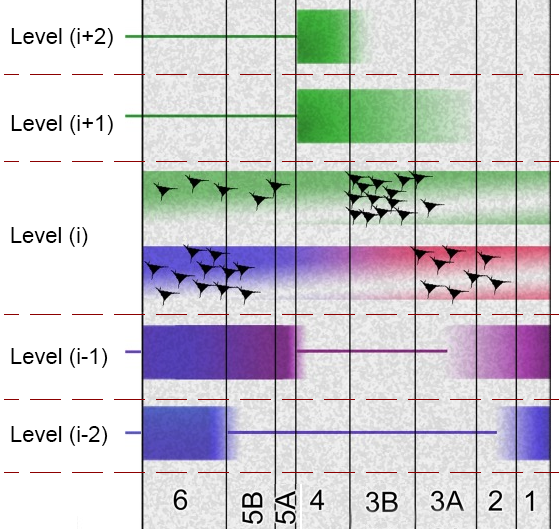
\includegraphics[width=0.5\textwidth, clip=true]{./Chapters/01_Introduction/Images/LaminarProcessing}
	\caption{Layer specific processing, adapted from Ship et al. (2013)\cite{Shipp2013}. From region $i$, there are feed forward connections (green) primarily targeting the middle layers in region higher in the cortical hierarchy ($i+1, i+2, \ell$). Feedback connections (blue, purple) target top and deep layers in lower regions in the hierarchy ($i-1, i-2, \ell$).}
	\label{fig:layerprocessing}
\end{figure}.

So the layers may give new information about the working of a single region, but may just as well be informative about cross-regional communication. There is 
The interregional connections have been described 

At the level of the microcircuit 

A massive network from connections to a large set 
\cite{Felleman1991}.



There is still a significant explanatory gap between the level of (cross-regional) prediction errors and the level of cognitive capacities. The cortical layer are right in the middle and 



 There is strong evidence that there are layer specific differences for (sensory) feed forward processes with respect to feedback processes.  Indeed, also functionally this seems to reflected in invasive electrical recordings in macaques \cite{Buffalo2011,Maier2010,Maier2011,VanKerkoerle2017}. 
 
 
Related with the layers of deep learning networks, although without direct proof \cite{Guclu}
 
interaction between brain regions
hierarchy study \cite{Michalareas2016}, DCM, inter region communication



%% I think here you should demonstrate more detailed knowledge of what these theories are. It isn't really enough to knock it off in a few lines. See some of the drawings in Felleman and van Essen, but also the publications of Shipp deserve a mention. Also it would be good to add some figures in here. 



For a small set of cognitive tasks, it is relatively straightforward to say if they are feed forward or feedback, but now think of more complicated processes: what would constitute as feed forward in language processing, decision making or memory? This is largely unknown and that is why it is of great interest to learn more about the laminar processing. It could shed light on a multitude of cognitive processes and open doors to a whole new type of information and new research in the brain \cite{Lawrence2017}. However, the greatest barrier is that neuronal communication is not easily measured. With fMRI, only a derivative of neuronal firing can be measured as changes in oxygen consumption. We will therefore first need to get a better understanding of what type of information it is that fMRI gives us.
%% This seems quite naiive, what are examples of feedforward tasks, how about within region interactions between layers? Is it worth mentioning predicitve coding?

\section*{MRI}
The basis of magnetic resonance imaging (MRI) is the phenomenon of nuclear magnetic resonance (NMR). In principle, this describes magnetic behaviour of protons and neutrons in terms of their \emph{quantum spin}: a preferred axis of rotation of an elementary particle. Normally, each spin has a random orientation of the axis of rotation. In the presence of a magnetic field, however, the spins will start precessing around the axis of the main magnetic field. The speed of rotation (angular frequency) will be directly proportional to the magnitude of the field, the Larmor frequency. In 1946, Felix Bloch and Edward Purcell %%These were completely independent groups
performed the first experiments in which they manipulated the spins with radio frequency (RF) pulses, for which they later received a Nobel prize \cite{Bloch1946}. They described how several magnetic properties of a material could be measured with this method, the relaxation times $T_1$ and $T_2$. %%I think the measurement of relaxation times came later, but I must admit I can't remember
These values describe the time it takes for spins in a certain material to go back to their rest position after they have been excited by an RF pulse for respectively the longitudinal magnetisation (aligned with the magnetic field) and the transverse magnetisation (perpendicular to the magnetic field). %%Only true for T1. T2 is only about phase coherence between spins.
Further development of the measurement technique allowed for a description of these properties as a function of two dimensional space,%% Lauterbur came up with projection imaging, and suggested using back projection to form images, something he had borrowed from X-ray CT.

 provided by Paul C. Lauterbur in 1973 \cite{Lauterbur1973}, for which he received a Nobel prize, thirty years later. This is still the basis of current MR imaging: a formalism in which the spatial frequencies of an image (\emph{k}-space) can be described as a time integral of an applied magnetic field (gradient), additional to the main magnetic field. %% Hohum. There are two references for k-space Twieg and I think a Swede (Sundgren). This came much later than Lauterbur. Lautrubur's projection formed the basis of gradient echo, but was emphatically not 2DFT! 
 This forms the basis for gradient echo pulse sequences.
The aforementioned $T_1$ and $T_2$ mechanism occurs as a random process of spins getting back to a rest equilibrium. There is an additional mechanism, $T_2^*$, in which the dephasing of the spins is not random but predictable, and thus reversible. After an RF pulse, spins start out by pointing in the same direction, but then fan out and start to dephase in clockwise or counter clockwise direction. Hence, the spins will cancel each other out, such that the signal decays much faster than $T_2$, but instead with $T_2^*$. However, their direction can be reversed (by a 180\textdegree RF pulse), such that they start to converge until they point in the same direction again to form a \emph{spin echo}. As a result gradient echo images are $T_2^*$-weighted and spin echo images are $T_2$-weigthed. In general, there is a variety of different acquisition sequences that all targeted different magnetic properties of the scanned object. 
%% As you mention them later it may be good to mention the principles of VASO and ASL.

\section*{Contrast Mechanisms}
Layers clearly differentiate in their functions, but measuring them is not easy. Especially in living humans this is hard, because the procedure is so invasive. It is ill-advised to stick electrodes in their heads, but what we can do is put them in an MRI scanner. An MRI scanner, however, cannot measure direct neuronal firing. Instead, it is susceptible to all kinds of magnetic properties of which three dimensional images can be made. Most notably, the magnetic susceptibility of red blood cells changes when they are oxygen rich or oxygen poor \cite{Ogawa1990}, which we call the Blood Oxygenation Level Dependant Signal, the BOLD signal. However, while there is little doubt that activation in a cortical region elicits a BOLD response, large parts of the biological mechanism behind it are still disputed. Most importantly, the extent to which the BOLD response reflects laminar specific activation is largely unknown.
%% Again a bit too simplistic. You can mention dia and paramagnetism

Figure~\ref{fig:microvasulature} shows the microvasculature of a small piece of visual cortex in a macaque. In red, the arterioles, small blood vessels that dive from the top of the cortex (the pial surface) downward to supply the whole grey matter with blood. The smallest vessels, the capillaries, relay the oxygen to the neurons in all cortical layers, such that deoxygenated hemoglobin is drained away by the veins (blue). The veins on top of the cortex can be an order of magnitude larger than the cortical veins, and conduct off the deoxygenated blood. This might make one appreciate the difficulty of extracting laminar specific signals with large signals of non-interest in the direct neighbourhood. 
\begin{figure}[!ht]
	\centering
	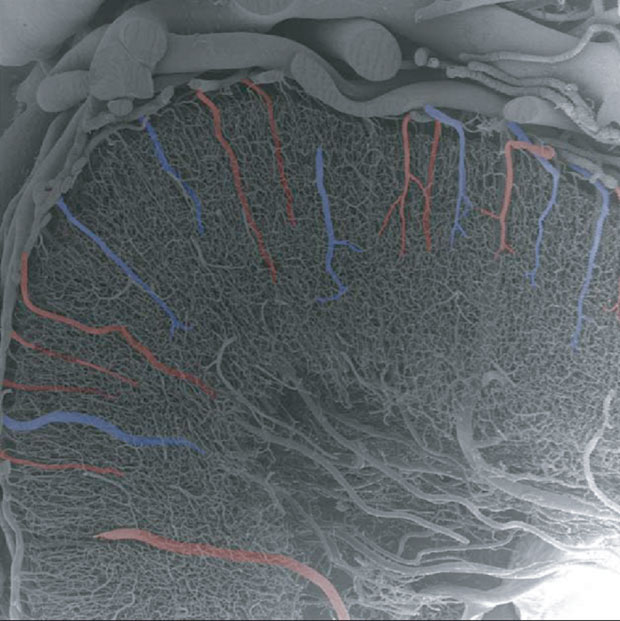
\includegraphics[width=0.9\textwidth, clip=true]{./Chapters/01_Introduction/Images/Microvasculature}
	\caption{The microvasculature of the visual cortex of a macaque \cite{Weber2008}. }
	\label{fig:microvasulature}
\end{figure}

But the level of blood oxygenation is not the only quantity that fluctuates as a result of cortical activation. 
%% This is leading in the wrong direction: the amount of deoxyhemoglobin is affected by CMRO2, CBF and CBV now it sounds like 'blood oxygentation' is a variable in its own right. 
More blood starts flowing (higher cerebral blood flow, CBF), vessels start dilating (more cerebral blood volume, CBV) and the consumption of oxygen increases (higher cerebral metabolic rate of oxygen, CMR$_{O2}$). These quantitative measures can be related to one another by the Davis model, save some free parameters that need to be empirically determined \cite{Davis1997}. 
%%^Why introduce the Davis model which we don't use?
However, the proposed equations hold for the cortical column in its entirety, but do not take into account potential layer specific differences. So while we cannot measure neuronal activation with MRI, the closest we can get is the traces in magnetic properties in the vasculature through BOLD, CBV, CBF, and CMRO$_{2}$. The extent to which these quantities vary as spatially specific as the level of the cortical layers is an outstanding question, however, and needs to empiraclly tested. Indeed, there are techniques to measure them, $T_2^*$-weighted imaging \cite{Norris2006} for BOLD, VASO for CBV \cite{Huber2018}, arterial spin labelling \cite{Grade2015} for CBV, and calibrated BOLD \cite{Blockley2013}) for CMRO$_{2}$. All vary in terms of sensitivity, specificity, and attainable resolution (spatial as well as temporal). The spatial resolution in combination with the type of experiment that is required for CBF and CMRO$_2$ measurements makes them poor candidates for human in vivo fMRI. It is mainly BOLD and CBV that have shown promising layer specific differences in animal experiments \cite{Lu2004,Zhao2006,Jin2008,Goense2012}. The main benefits of VASO compared to BOLD are its quantifiability \cite{Lu2003} and local specificity \cite{Jin2006}, whereas BOLD has higher sensitivity and speed \cite{Huber2018}. %%The comparison with GE BOLD in Renzo's paper is not really fair.

Our main goal was to investigate the possibilities of laminar analysis in standard experiments on humans, and hence chose to use the BOLD signal as our signal of interest. 
%%I'm not convinced by the order you have chosen. We get a cursory intro to BOLD, then VASO and ASL and then we return to BOLD but it takes some time to get to the differences gradient-/spin-echo. Why not first do BOLD 'properly' and then you can compare SE/GE with VASO/ASL?
Fundamentally, the BOLD signal arises as a consequence of magnetic field perturbations arising from desoxyhemoglobin molecules \cite{Norris2006}. These changes extend beyond the blood vessel into the tissue and drop off as a function of field strength, the orientation of the vessel, and the vessel diameter as well as the concentration of deoxyhemoglobin. From the time that the molecules are excited until the time of the echo, molecules in the tissue move around the vasculature. If the trajectory of a molecule in this time is small compared to the vessel size (and hence compared to the drop-off), there is little change in its surrounding magnetic field and the effect is reversible, a static effect. If on the other hand the molecule's trajectory is large, its surrounding magnetic field changes more drastically and unpredictably, such that the effect is irreversible and dynamic. These two contrast mechanisms are the static and dynamic extravascular effect. The magnetic field perturbations around the vessels scale linearly with field strength, so the trajectory of a molecule relative to the perturbations is much greater at 7 Tesla than at 1.5 Tesla. Thus, the dynamic extravascular effect increase with field strength. The remaining static effect at 7 Tesla is thus very specific, but detecting it requires high sensitivity \cite{Panchuelo2014}. %%Static goes linearly with B0, dynamic quadratically.

An additional source of BOLD contrast is the intravascular effect. The magnetic field inside the vessel is slightly different from the surrounding tissue because of the amount of desoxyhemoglobin. As a result, the signal will start to dephase with respect to the extravascular signal. This is can be reversed because it is constant over time and is called the static intravascular effect. The last contrast mechanism that contributes to the BOLD signal is disputed in origin. This is irreversible (dynamic) intravascular dephasing and has to do with the random movement of water molecules within red blood cells. It is either due to these water molecules interacting with the deoxyhemoglobin, or with the diffusion in and out of the cells, but no experiment to date has been able to tease the two mechanisms apart.
%%Good to explain that of four contrast mechanisms two are 'invisible' to SE, and why that is postulated to give better intrinsic spatial resolution at UHF.
Even given these four contrast mechanisms, it is still an outstanding question in what proportions they proliferate in measurements. This may even vary at the laminar level, as the deoxyhemoglobin from deeper layers flows upward to the top layers. The strengths of these effects have been modelled for both spin echo and gradient echo and suggest that most of the signal produced in a layer is also visible in that layer \cite{Markuerkiaga2016,Uludag2017}. For spin echo this effect is minimal, while gradient echo has a tail that extents to more superficial layers, but at a gain of sensitivity. A range of laminar profiles has been found using spin echo (e.g. \cite{Zhao2004,Harel2006,Goense2006}), gradient echo (e.g. \cite{Polimeni2010,DeMartino2013,Chen2013}) or a combination of both, GRadient A Spin Echo (GRASE) \cite{Olman2012,DeMartino2013}.

Choosing a sequence requires carefully balancing the advantages and disadvantages against each other. We here chose to use gradient echo to investigate the laminar BOLD signal for its higher sensitivity and at a field strength of 7 Tesla for high specificity. The potential downside of this is the susceptibility to the larger veins on top of the cortex that might obscure smaller effects \cite{Barth2007}. While the exact origins of the BOLD signal are unknown, there is strong evidence that the BOLD signal has a laminar footprint \cite{Logothetis2001}. Although some results from animal studies suggest that the effects may be visible at a higher temporal resolution than human in vivo MRI can achieve \cite{Yu2014,OHerron2016}. With the many uncertainties and the small size of the potential effect, it is clear that any potential effect can only be picked up with powerful methods that address as many sources of noise as possible. 
%%It may be good to discuss some of the characteristics of 3D EPI and also what you can expect at different field strengths as you have looked at both 3T and 7T data.

\section*{Methods}
After covering the fundamentals of measurement techniques, it is clear what types of information may be expected to be present in the data. Getting out the relevant information, however, is at least as complicated. The brain is a highly convoluted structure that we are trying to describe and visualise by means of cubic voxel rasters. The first problem we encounter is a geometrical one: how do we attach a brain location to voxels in space? This can be done by making a \emph{cortical reconstruction} on a high resolution brain scan \cite{Dale1999,Bazin2012} with a very clear contrast between the white matter and grey matter as seen in Figure~\ref{fig:mybrain}. The distinction between white and grey matter is clear enough to draw a three dimensional boundary on both side of the grey matter: on the white matter boundary and on the pial surface, the separation between the grey matter and the cerebrospinal fluid (CSF).
\begin{figure}[!ht]
	\centering
	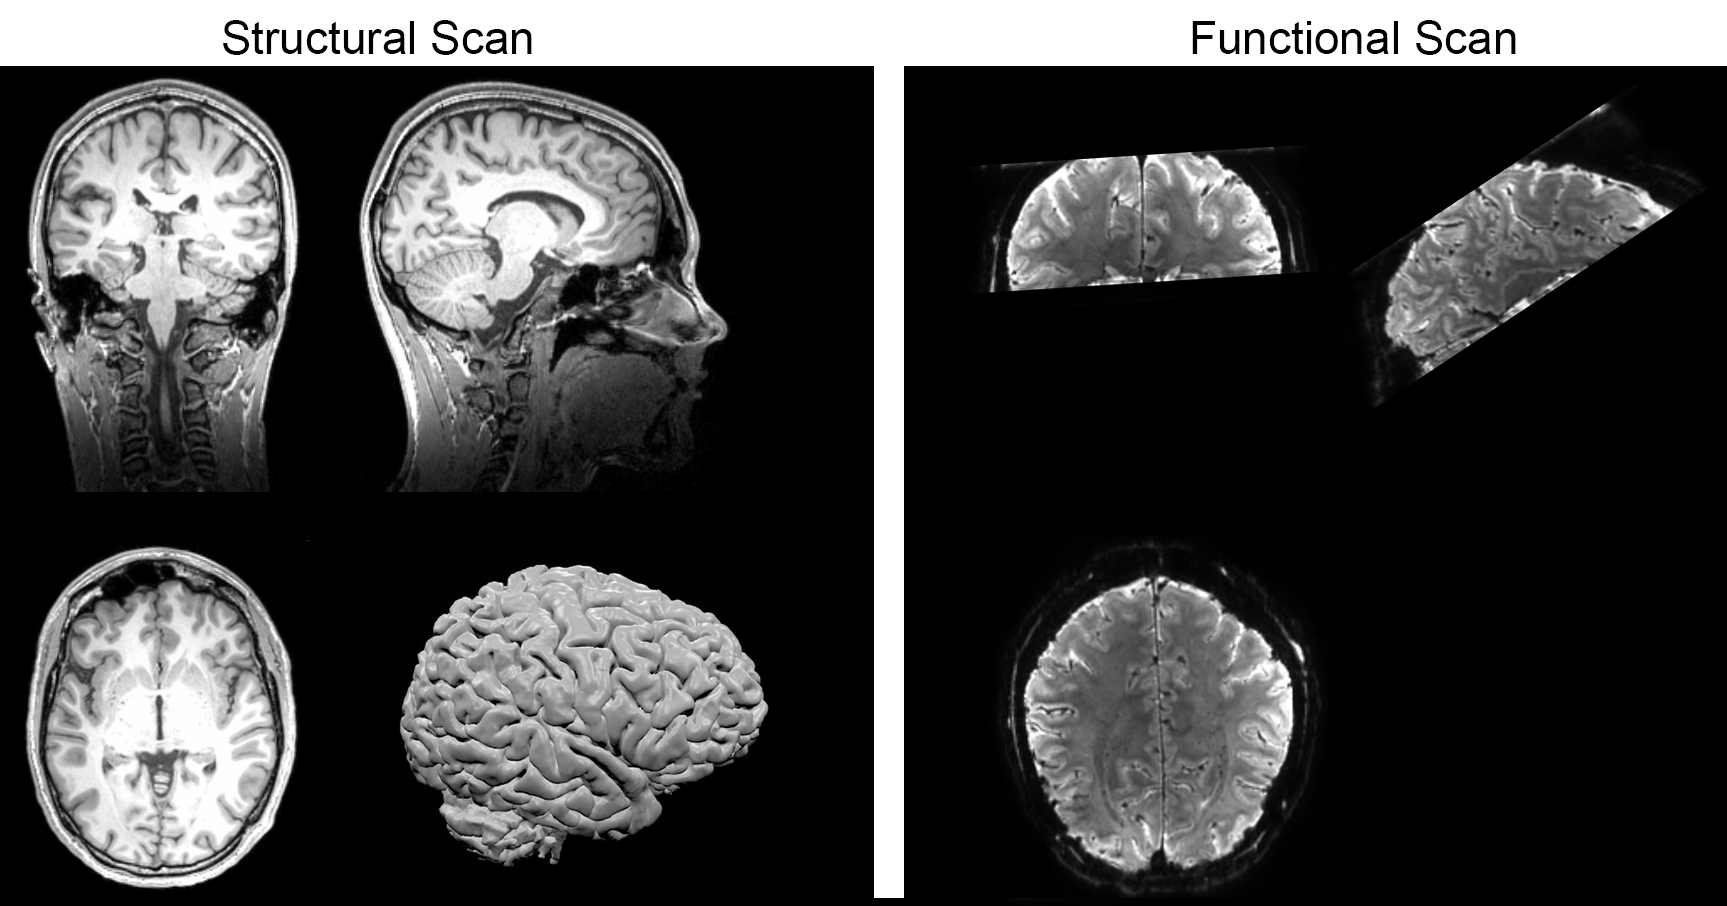
\includegraphics[width=0.99\textwidth, clip=true]{./Chapters/01_Introduction/Images/MyBrain}
	\caption{An example of a structural and functional brain scan. On the left, the structural scan has high anatomical contrast and sharp differences between the white matter and grey matter. The contrast is sharp enough to make a three dimensional reconstruction of the brain (lower right corner). On the right, a functional image is shown. The anatomical contrast is much weaker, but it can be acquired quickly and the contrast is susceptible to slight changes in blood deoxyhemoglobin, related to oxygen consumption on neuronal activation.}
	\label{fig:mybrain}
\end{figure}

The cortical reconstruction is very informative about the shape of the brain and potentially also about the layers: One could imagine different layers to be described as intermediate surfaces between both outer boundaries of which the locations can be used to then sample the cortical layers \cite{Koopmans2011,Polimeni2010,DeMartino2013}. This description allows for all sorts of surface based calculations \cite{Fischl2000,Bazin2012} and for example allows us to take into account a more naturalistic flow of the cortical layers \cite{Bok1929,Waehnert2014}. Along the many curves of the cortex, the layers approximately conserve volume for a given cortical column. Taking this into account can provide a clear advantage in high resolution laminar analysis.
%%At some point it would be good to describe what the structural scans look like, which contrasts are available, and how they differ from the functional scans. 

The cortical reconstruction can be made on a dedicated high resolution high contrast scan, but this does not yet give functional information. First, the cortical surfaces need to be `coregistered' with the functional data and brought into the same analysis space. Unfortunately, this is made considerably more difficult by two main factors. First, the contrast and resolution of standard gradient echo functional data is poor, so there is not a lot of information on which to base a good coregistration. Secondly, when `echo planar imaging' (EPI) is used, a fast acquisition scheme to collect data, the data will to some extent be geometrically distorted. The reason is that the scanner magnetic field is not everywhere exactly equal. When we talk about a scanner with a field strength of 7 Tesla, it means there should be a stable static magnetic field of that strength in the centre of the scanner. However, because the presence of a human body perturbs the field, it is not as homogeneous as one might desire. Small perturbations can be corrected by \emph{shimming}, applying an additional magnetic field to compensate for the inhomogeneities. However, this is not accurate enough to correct all deviations and the inhomogeneities need not even be constant over time. As mentioned before, MRI is based on spins precessing at a frequency that is proportional to the field strength. If the field is slightly higher or lower, the spins in that area precess slightly faster or slower. It was noted that MRI measures spatial frequencies of an image, assuming a constant magnetic field. So one could imagine that as a direct result of the Fourier shift theorem, spins that precess faster or slower are instead displaced in the resulting image. Since the displacement is field strength dependent, distortions are more pronounced at higher fields. They can easily be of the order of several millimetres, which comes down to a shift of the size of the entire cortex. So extreme care must be taken in aligning scans properly and thoroughly checking the correctness of the cortical surface in the regions that one wants to analyse. %%I think you can improve this explanation, for example why is distortion only along phase-encoding axis. 

There is a wide variety of other potential sources of noise that can contaminate the (laminar) signal. Participants in a study will move several millimetres, breathe and have a heartbeat that is clearly visible in the signal, people may have lapses in their attention, may even fall asleep to the rhythm of the helium pump, et cetera. Many operations are performed on the data to remove as many sources of noise as possible and this creates long analysis pipelines. This makes the process of doing fMRI analysis difficult at the conceptual level, and may also create a logistical nightmare: different software packages, programming languages, data types, data representations, and different styles of programming. As a result, it is understandable that the reproducibility of fMRI results can be low \cite{Nosek2015,Gorgolewski2016a}. We here took care to build and use all tools as reproducibly as possible and to provide all data openly, accompanied with the scripts to generate the results.

\section{Layers Analysis in human FMRI}


statistical problem

pulsation of the brain 

%%%%
In addition, 



Imaging flying in loud helicopter above a large highway crossing, and with a microphone you try to pick up the sound of the cycling lane.

Picking up the footsteps of a pedestrian on the side  road, next to a loud highway when an 



While it is known in which layers are intially targeted by feedback and feed foward signals, little is known about their further processing. There is evidence that excitatory neurons may quickly redistribute input from the thalamus by means of their local axonal collaterals \cite{Guy2017,ReyesPuerta2015}. As a result, cortical activity may nearly instantaneously spread over several layers and columns, to the detriment of laminar specificity of the BOLD signal.

\cite{Maass2014}


We did not discuss variability in thickness of the layers

\cite{Heinzle}

\cite{Renzo}

accelarated imaging, GRAPPA, SENSE


Needle in a haystack on a windy day


2D versus 3D acquisition

k-space equation



